\section{Mật mã đường cong elliptic}
\subsection{Khái niệm hệ mật mã và các loại hệ mật mã}

\subsubsection{Khái niệm hệ mật mã}
Hệ mật mã là một tập hợp các phương pháp và kỹ thuật được sử dụng để 
bảo vệ thông tin truyền qua các kênh truyền thông không an toàn. Nó 
bao gồm các phương pháp mã hóa và giải mã thông tin để chỉ cho người 
dùng hợp lệ đọc được thông tin. Đồng thời, hệ mật mã cũng bao gồm các 
kỹ thuật xác thực người dùng và đảm bảo tính toàn vẹn của thông tin.

Hệ mật mã là hệ thống bao gồm các thành phần như sau:
\begin{itemize}
    \item[-] Bản rõ là tập hợp hữu hạn các thông tin cần được bảo mật.
    \item[-] Bản mã là tập hợp hữu hạn các thông tin được mã hóa từ bản rõ.
    \item[-] Một tập hợp các khóa: khoá công khai $K_{pub}$ và khoá bí mật $k_{pri}$.
    \item[-] Một thuật toán mã hóa $E$, mã hoá bản rõ thành bản mã.
    \item[-] Một thuật toán giải mã $D$, giải mã bản mã thành bản rõ gốc.
\end{itemize}

Quy trình mã hoá và giải mã được thể hiện qua sơ đồ sau:
\begin{figure}[h]
    \centering
    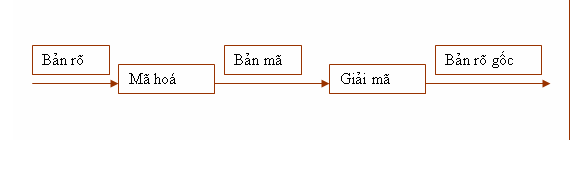
\includegraphics[width=0.5\textwidth]{images/encrypt-decrypt.png}
    \caption{Quy trình mã hoá và giải mã}
    \label{fig:encrypt-decrypt}
\end{figure}

Tính chất cơ bản của mật mã:
\begin{itemize}
    \item[-] Tính bí mật: đảm báo tính bí mật của dữ liệu mà mình gửi đi và
        chỉ những người nắm giữ khoá mới có thể đọc được nội dung.
    \item[-] Tính toàn vẹn: đảm bảo dữ liệu không bị mất mát hoặc chỉnh sửa 
    trong quá trình gửi và nhận mà không bị phát hiện.
    \item[-] Tính xác thực: đảm bảo danh tính của thực thể được xác minh.
    \item[-] Tính không thể chối từ:  đảm bảo người gửi không thể phủ nhận
    thông tin mình gửi đi.
\end{itemize}


\subsubsection{Các loại hệ mật mã}
Các hệ mật mã được chia thành hai loại chính: 
\begin{itemize}
    \item[-] Hệ mật mã đối xứng
    \item[-] Hệ mật mã bất đối xứng
\end{itemize}

a) Hệ mật mã đối xứng

Mật mã đối xứng là một hệ mật mã sử dụng cùng một khóa để mã hóa và giải mã thông tin.
Vì vậy nên khoá bí mật phải giữ an toàn và không được chia sẻ với bất kỳ ai.

Một số hệ mật mã khóa đối xứng hiện đại hay được sử dụng là DES, AES, RC4, RC5,...

Hệ mật sẽ bao gồm:
\begin{itemize}
    \item[-] Bản rõ (M)
    \item[-] Bản mã (C)
    \item[-] Khoá (K)
    \item[-] Mã hoá (E): $C = E(K,M)$
    \item[-] Giải mã (D): $M = D(K,C) = D(K,E(K,M))$
\end{itemize}

Vì dùng chung một khoá nên mật mã đối xứng có một số mặt hạn chế như:
\begin{itemize}
    \item[-] Nếu bị đánh cắp hoặc mất khoá thì thông tin cần gửi sẽ bị lộ
    \item[-] Khoá do bên thứ 3 tạo và phải gửi từ bên người gửi đến người nhận, 
    cần phải có một kênh truyền thông an toàn để truyền khoá. Việc đảm bảo khoá 
    không bị lộ khi truyền đi cũng là vấn đề lớn.
    \item[-] Truyền tin giữa các nhóm nhiều người cần 1 lượng lớn khoá, vì 3 người 
    thì không thể dùng chung khoá, giữa 2 người phải có khoá riêng để đảm bảo rằng
    thông tin truyền đi giữa 2 người không bị lộ cho người thứ 3.
    \item[-] Thông tin truyền đi có thể bị sửa đổi vì không có cơ chế xác thực.    
\end{itemize}

Chính vì những nhược điểm như trên nên hệ mật mã bất đối xứng ra đời.

b) Hệ mật mã bất đối xứng

Hệ mã bất đối xứng (hệ mã khoá công khai) là hệ mật mã sử dụng hai khóa khác nhau để mã hóa và giải mã thông tin.
Khoá công khai dùng để mã hoá thông tin và khoá bí mật dùng để giải mã thông tin. Khoá công khai được công khai 
cho tất cả mọi người, còn khoá bí mật thì người nhận nắm giữ.


Hệ mật sẽ bao gồm:
\begin{itemize}
    \item[-] Bản rõ (M)
    \item[-] Bản mã (C)
    \item[-] Khoá (K): 
        \\+ Khoá công khai ($K_{pub}$)
        \\+ Khoá bí mật ($K_{pri}$) 
    \item[-] Mã hoá (E): $C = E(K_{pub},M)$
    \item[-] Giải mã (D): $M = D(K_{pri},C) = D(K_{pri},E(K_{pub},M))$
\end{itemize}

Một số phương pháp sử dụng để trao đổi khoá trong có hệ mật là:
\begin{itemize}
    \item[-] Trao đổi khoá Diffie-Hellman
    \item[-] Trao đổi khoá RSA
    \item[-] Trao đổi khoá ElGamal
\end{itemize}

trong khoá luận này, em sẽ tập chung vào trao đổi khoá Diffie-Hellman.
\subsection{Trao đổi khoá Diffie-Hellman}

Thuật toán trao đổi khóa Diffie-Hellman giải quyết tình huống sau. Alice và
Bob muốn chia sẻ một khóa bí mật để sử dụng trong mật mã đối xứng, nhưng
phương thức liên lạc của họ không an toàn. Mọi thông tin mà họ trao
đổi đều được quan sát bởi Eve - kẻ tấn công. Làm sao để Alice và Bob có
thể chia sẻ khóa mà Eve không biết? Độ khó của bài toán logarit rời
rạc trong $\mathbb{F}^*_p$ đã đưa ra một giải pháp.

% Thuật toán Trao đổi khoá Diffie - Hellman được tóm tắt ở bảng sau

% \begin{tabular}{|c|c|}
% 	\hline
% 	\multicolumn{2}{Tạo tham số công khai}                                                                                                     \\
% 	\hline
% 	\multicolumn{2}{c}{Một bên chọn và công khai một số nguyên tố $p$ (lớn) và một số nguyên $g$ có bậc nguyên tố lớn trong $\mathbb{F}^*_p$}. \\
% 	\hline
% 	\hline
% 	\multicolumn{2}{c}{Thực hiện tính toán bí mật}                                                                                             \\
% 	Alice                         & Bob                                                                                                        \\
% 	\hline
% 	Chọn bí mật một số nguyên $a$ & Chọn bí mật một số nguyên $b$                                                                              \\
% 	Tính $A \equiv g^a \pmod{p}$  & Tính $B \equiv g^b \pmod{p}$                                                                               \\
% 	\hline
% 	\hline
% 	\multicolumn{2}{c}{Trao đổi giá trị công khai}                                                                                             \\
% 	Alice gửi $A$ cho Bob         & $\longrightarrow A$                                                                                        \\
% 	$B \longleftarrow$            & Bob gửi $B$ cho Alice                                                                                      \\
% 	\hline
% 	\hline
% 	\multicolumn{2}{c}{Tiếp tục thực hiện tính toán bí mật}                                                                                    \\
% 	Alice                         & Bob                                                                                                        \\
% 	\hline
% 	Tính $B^a \pmod{p}$           & Tính $A^b \pmod{p}$                                                                                        \\
% 	Khóa bí mật của cả hai là giá trị $B^a \equiv (g^b)^a \equiv g^{ab} \equiv (g^a)^b \equiv A^b \pmod{p}$
% \end{tabular}

Đầu tiên, Alice và Bob thống nhất sử dụng một số nguyên tố $p$ và một số nguyên khác không $g$  theo modulo $p$. 
Tiếp theo, Alice bí mật chọn một số nguyên $a$ và không cho ai biết. Cùng lúc đó, Bob cũng bí mật chọn một số nguyên $b$.
Alice và Bob sử dụng những số bí mật của họ và tính
$$\underbrace{A \equiv g^a \pmod{p}}_{\text{Alice tính}} \text{ và } \underbrace{B \equiv g^b \pmod{p}}_{\text{Bob tính}}$$.

Sau đó, họ trao đổi với nhau giá trị vừa tính được, Alice gửi $A$ cho Bob và Bob gửi $B$ cho Alice. 
Cuối cùng, Bob và Alice tiếp tục sử dụng những số bí mật mà họ đã chọn ở bước trước đó, và tính
$$\underbrace{A' \equiv B^a \pmod{p}}_{\text{Alice tính}} \text{ và } \underbrace{B' \equiv A^b \pmod{p}}_{\text{Bob tính}}$$.

$A'$ và $B'$, là bằng nhau, vì:
$$A' \equiv B^a \equiv (g^a)^b \equiv g^{ab} \equiv (g^b)^a \equiv A^b \equiv B' \pmod{p}.$$

Giá trị này là khóa mà cả hai cùng chấp nhận sử dụng.

Kẻ tấn công biết được giá trị $p,g,g^a \mod p, g^b \mod p $ nhưng không 
tính toán được khoá $k = g^{ab} \mod p$. Đây là một bài toán khó giải 
trong thời gian đa thức. \cite{elliptic}

\subsection{Mật mã đường cong elliptic}
\subsubsection{Khái niệm đường cong elliptic}

Một \textit{đường cong Elliptic} là tập nghiệm của một phương trình có dạng
$$Y^2 = X^3 + AX + B$$ cùng với một điểm $\mathcal{O}$ ở vô cùng, trong đó hằng số $A$ và $B$ thỏa mãn
$$ 4A^3 + 27B^2 \neq 0$$
Các phương trình thuộc loại này được gọi là \textit{phương trình Weierstrass}. 
Đồ thị của đường cong elliptic có dạng đối xứng qua trục hoành. \cite{elliptic}

Điểm $\mathcal{O}$ là điểm đặc biệt của đường cong elliptic, nó không thuộc đường cong.
Khi ta cộng điểm $P$ với một điểm $P'$ đối xứng với $P$ qua đường cong thì ta có:

$$ P \oplus P' = \mathcal{O}$$

Hai ví dụ cho đường cong elliptic:
$$ E_1: Y^2=X^3-3X+3 $$ và $$ E_2: Y^2=X^3-5X+5 $$ được minh họa ở \hyperref[fg:fg1]{Hình I.2}

\begin{figure}[H]

	\label{fg:fg1}
	\begin{minipage}{0.4\textwidth}
		\centering
		\begin{tikzpicture}[scale = 0.5, line cap=round,line join=round,>=triangle 45,x=1cm,y=1cm]
			\begin{axis}[
					x=1cm,y=1cm,
					axis lines=middle,
					xmin=-5.912600967627929,
					xmax=5.112504977805202,
					ymin=-5.000000419005899,
					ymax=5.000000419005899,
					xtick={-5,-4,...,5},
					ytick={-5,-4,...,5},]
				\clip(-5.912600967627929,-5.000000419005899) rectangle (10.112504977805202,5.000000419005899);
				\draw[line width=2pt,color=blue,smooth,samples=100,domain=-2.1038033040947663:10.112504977805202] plot(\x,{sqrt((\x)^(3)-3*(\x)+3)});
				\draw[line width=2pt,color=blue,smooth,samples=100,domain=-2.1038033040947663:10.112504977805202] plot(\x,{0-sqrt((\x)^(3)-3*(\x)+3)});
			\end{axis}
		\end{tikzpicture}
	\end{minipage}
	\hfill
	\begin{minipage}{0.4\textwidth}
		\centering
		\begin{tikzpicture}[scale = 0.5, line cap=round,line join=round,>=triangle 45,x=1cm,y=1cm]
			\begin{axis}[
					x=1cm,y=1cm,
					axis lines=middle,
					xmin=-5.912600967627929,
					xmax=5.112504977805202,
					ymin=-5.000000419005899,
					ymax=5.000000419005899,
					xtick={-5,-4,...,5},
					ytick={-5,-4,...,5},]
				\clip(-5.912600967627929,-5.000000419005899) rectangle (10.112504977805202,5.000000419005899);
				\draw[line width=2pt,color=blue,smooth,samples=100,domain=-2.791287717641796:0.9999998864501113] plot(\x,{sqrt(abs((\x)^(3)-6*(\x)+5))});
				\draw[line width=2pt,color=blue,smooth,samples=100,domain=1.791293439719924:10.112505461619168] plot(\x,{sqrt(abs((\x)^(3)-6*(\x)+5))});
				\draw[line width=2pt,color=blue,smooth,samples=100,domain=-2.791287717641796:0.9999998864501113] plot(\x,{0-sqrt(abs((\x)^(3)-6*(\x)+5))});
				\draw[line width=2pt,color=blue,smooth,samples=100,domain=1.791293439719924:10.112505461619168] plot(\x,{0-sqrt(abs((\x)^(3)-6*(\x)+5))});
			\end{axis}
		\end{tikzpicture}
	\end{minipage}
	\caption{Đường cong elliptic $E_1$ và $E_2$}
\end{figure}



\subsubsection{Các phép toán trên đường cong elliptic}
a) Phép cộng 

Luật cộng trên $E$ được định nghĩa như sau:

Cho 2 điểm $P$ và $Q$ là 2 điểm thuộc $E$.
$L$ là đường thẳng nối $P$ và $Q$, hoặc là đường tiếp tuyến của $E$ tại $P$ nếu $P=Q$.
Khi đó, giao điểm của $E$ và $L$ là ba điểm $P$, $Q$ và $R$, với $\mathcal{O}$
được hiểu là điểm nằm trên mọi đường thẳng đứng. $R=(a,b)$, tổng của $P$ và $Q$
là điểm $R'=(a,-b)$. Tổng này được ký hiệu là $P \oplus Q$, có thể viết đơn giản $P+Q$.

Luật cộng có thể được minh hoạ qua hình vẽ sau:

\begin{figure}[H]
	\label{fg:fg2}
	\centering
	\resizebox{0.5\textwidth}{!}{%
	\begin{tikzpicture}[line cap=round,line join=round,>=triangle 45,x=1cm,y=1cm]
		\clip(-5.736430725533388,-5.733053262983473) rectangle (5.923722428745249,5.872549467181578);
		\draw[line width=0.8pt,color=blue,smooth,samples=100,domain=-2.103803291543122:5.923722428745249] plot(\x,{sqrt(abs((\x)^(3)-3*(\x)+3))});
		\draw[line width=0.8pt,color=blue,smooth,samples=100,domain=-2.103803291543122:5.923722428745249] plot(\x,{0-sqrt(abs((\x)^(3)-3*(\x)+3))});
		\draw [line width=0.8pt,domain=-5.736430725533388:5.923722428745249] plot(\x,{(--2.3486301286669415-0.40680839258599555*\x)/1.3559822370127241});
		\draw [line width=0.8pt,dotted] (1.4459883083356893,-1.9982396827947813)-- (1.4459883083356893,1.9982396827947813);
		\begin{scriptsize}
			\draw[color=black] (-1.9451762496392822,0.28794979855338965) node {$E$};
			\draw [fill=black] (0,1.7320508075688772) circle (2pt);
			\draw[color=black] (0.2232031088756924,1.9926505521028977) node {$Q$};
			\draw [fill=black] (-1.3559822370127241,2.1388592001548727) circle (2pt);
			\draw[color=black] (-1.1405574939639143,2.4017787329547793) node {$P$};
			\draw[color=black] (-5.463678604965468,2.8700487609709) node {$L$};
			\draw [fill=black] (1.4459883083356893,1.2982396827947813) circle (2pt);
			\draw[color=black] (1.777890196112844,1.5698847652226198) node {$\ R$};
			\draw [fill=black] (1.4459883083356893,-1.2982396827947813) circle (2pt);
			\draw[color=black] (2.4324952854758553,-1.0348979862010284) node {$R' = P \oplus Q$};
		\end{scriptsize}
	\end{tikzpicture}
	}%
	\caption{Phép cộng trên đường cong elliptic}
\end{figure}

Nếu ta muốn cộng điểm $P$ với chính nó, thì ta lấy đường thẳng L là tiếp tuyến của đồ thị
qua điểm $P$.

Kết quả được minh hoạ trong hình vẽ sau:

\begin{figure}[H]
	\label{fg:fg3}
	\centering
	\resizebox{0.5\textwidth}{!}{%
	\begin{tikzpicture}[line cap=round,line join=round,>=triangle 45,x=1cm,y=1cm]
		\clip(-5.736430725533388,-5.733053262983473) rectangle (5.923722428745249,5.872549467181578);
		\draw[line width=0.8pt,color=blue,smooth,samples=100,domain=-2.103803291543122:5.923722428745249] plot(\x,{sqrt(abs((\x)^(3)-3*(\x)+3))});
		\draw[line width=0.8pt,color=blue,smooth,samples=100,domain=-2.103803291543122:5.923722428745249] plot(\x,{0-sqrt(abs((\x)^(3)-3*(\x)+3))});
		\draw [line width=0.8pt,domain=-5.736430725533388:5.923722428745249] plot(\x,{(-0.011820467984078764-0.0023798531917433863*\x)/-0.0040177629872759635});
		\draw [line width=0.8pt,dotted] (3.06684049847989,-5.458642606222206)-- (3.06684049847989,5.458642606222206);
		\begin{scriptsize}
			\draw[color=black] (-1.9451762496392822,0.28794979855338965) node {$E$};
			\draw [fill=black] (-1.36,2.1364793469631294) circle (2pt);
			\draw [fill=black] (-1.3559822370127241,2.1388592001548727) circle (2pt);
			\draw[color=black] (-1.1405574939639143,2.4017787329547793) node {$P$};
			\draw[color=black] (-5.463678604965468,-0.10754077627009614) node {$L$};
			\draw [fill=black] (3.06684049847989,4.758642606222206) circle (2pt);
			\draw[color=black] (3.400765313491976,5.020199090406824) node {$\ R$};
			\draw [fill=black] (3.06684049847989,-4.758642606222206) circle (2pt);
			\draw[color=black] (4.0553704028549875,-4.4988499174136285) node {$R' = P \oplus P = 2P$};
		\end{scriptsize}
	\end{tikzpicture}
	}%
	\caption{Phép cộng điểm P với chính nó}
\end{figure}


\begin{theorem}[Thuật toán cộng đường cong Elliptic]
	\label{th:th2}
	Cho
	$$E:Y^2 = X^3 + AX + B$$
	là một đường cong elliptic và $P_1$  và $P_2$ là hai điểm trên $E$.
	\begin{enumerate}
		\item Nếu $P_1 = \mathcal{O}$ thì $P_1 + P_2 = P_2$.
		\item Ngược lại, nếu $P_2 = \mathcal{O}$ thì $P_1 + P_2 = P_1$.
		\item Ngược lại, viết $P_1 = (x_1, y_2)$ và $P_2 = (x_2, y_2)$.
		\item Nếu $x_1 = x_2$ và $y_1 = -y_2$ thì $P_1 + P_2 = \mathcal{O}$.
		\item Nếu không, định nghĩa $\lambda$ bởi
		      $$ \lambda = \begin{cases}
				      \frac{y_2-y_1}{x_2 - x_1} & \text{nếu } P_1 \neq P_2 \\
				      \frac{3x_1^2 + A}{2y_1}   & \text{nếu } P_1 = P_2.
			      \end{cases} $$
		      Và ta có $P_1 + P_2 = (x_3, y_3)$, trong đó:
		      $$x_3 = \lambda^2 - x_1 - x_2 \ \ \  \text{ và } \ \ \  y_3 = \lambda(x_1 - x_3) - y_1.$$
	\end{enumerate}
\end{theorem}


b) Phép nhân

Phép nhân $P$ với một số nguyên $n$ được định nghĩa bởi 
$$nP = P + P + \cdots + P$$
với $n$ lần phép cộng.

\subsubsection{Đường cong elliptic trên trường hữu hạn}
Các ứng dụng về mật mã của đường cong Elliptic đa số chỉ sử dụng các đường cong trên
trường hữu hạn.

\begin{definition}
    	Trường là một tập hợp K có nhiều hơn một phần tử, được định nghĩa hai phép toán cộng và nhân,
    	ký hiệu bởi dấu $(+)$ và dấu $(.)$. Trường thỏa mãn các tính chất của số học.
\end{definition}

\begin{definition}
	Trường hữu hạn (còn gọi là trường Galois) là những trường có hữu hạn số phần tử.
	Bậc của một trường hữu hạn là số phần tử của nó, là số nguyên tố hoặc lũy thừa nguyên tố.
\end{definition}
Trường hữu hạn là cơ bản trong một số lĩnh vực toán học và khoa học máy tính,
bao gồm lý thuyết số, hình học đại số, lý thuyết Galois, hình học hữu hạn, mật mã và lý thuyết mã hóa.

Đường cong elliptic $E$ trên trường hữu hạn $\mathbb{F}_q$ là một phương trình có dạng:
$$E: Y^2 = X^3 + AX + B\ \text{với các hằng số}\ A, B \in F_p\ \text{thỏa mãn}\ 4A^3 + 27B^2 \neq 0$$

Tập hợp các điểm trên $E$ có toạ độ thuộc $\mathbb{F} _p$ được kí hiệu bởi
$$E(F_p) = \{(x, y) : x, y \in \mathbb{F}_p\ \text{thỏa mãn}\ y^2 = x^3 + A x + B\} \cup \mathcal{O}$$

\subsubsection{Khái niệm mật mã đường cong elliptic}
Mật mã đường cong elliptic (ECC) 
là một phương pháp mã hóa và giải mã thông tin bằng cách sử dụng các 
điểm trên đường cong elliptic. ECC được sử dụng để đảm bảo tính bảo 
mật và an toàn trong các ứng dụng mật mã, như mã hóa thông tin, xác thực người dùng, và tạo chữ ký số.

Trao đổi khóa Diffie - Hellman trên elliptic, thay thế bài toán logarit rời
rạc cho trường hữu hạn $F_p$ bằng bài toán logarit rời rạc cho đường cong elliptic $E(F_p)$.
Đây là các bài toán khó có thể giải quyết trong thời gian đa thức. Phù 
hợp để sử dụng trong các ứng dụng mật mã.

a) Trao đổi khoá Diffie - Hellman trên đường cong elliptic

	Alice và Bob cùng đồng ý sử dụng một đường cong elliptic $E (\mathbb{F}_p)$ và một điểm $P \in E (\mathbb{F}_p)$.
	Alice bí mật chọn một giá trị $n_A$, Bob chọn một giá trị $n_B$. Cả hai sử dụng số bí mật của họ và tính
$$\underbrace{Q_A = (n_AP)}_{\text{Alice tính}} \text{ và } \underbrace{Q_B = (n_BP)}_{\text{Bob tính}}$$

Sau đó, họ trao đổi với nhau giá trị vừa tính được, Alice gửi $Q_A$ cho Bob và Bob gửi
$Q_B$ cho Alice. Sau đó tính $n_A Q_B$ và $ n_BQ_A $.
Và họ có khóa bí mật chung
$$ n_AQ_B = (n_An_B)P = n_BQ_A,$$

Giống như bài toán logarit rời rạc trên trường hữu hạn, bài toán logarit rời rạc trên đường cong elliptic 
cũng là một bài toán khó. 

Hiện nay, thuật toán phổ biến để giải quyết bài toán logarit rời rạc 
trên đường cong elliptic là thuật toán Pollard's rho và thuật toán 
đặc biệt hơn là thuật toán số học đại số đường cong elliptic (ECDLP).

Thuật toán Pollard's rho được sử dụng để tìm giá trị bí mật của 
logarit rời rạc trên đường cong elliptic bằng cách sử dụng phép 
nhân trên đường cong để tìm kiếm các chu kỳ lặp lại. Thuật toán này 
có độ phức tạp tính toán khoảng $O(\sqrt n)$, trong đó $n$ là số lượng 
phần tử trong đường cong.

Vậy nên để đảm bảo độ bảo mật và tính khó tính toán cho bài toán trên,
ta sử dụng đường cong elliptic có số phần tử lớn, hay chọn $p$ là một
số nguyên tố lớn, và chọn 1 đường cong elliptic trên trường hữu hạn $F_p$. \cite{Elliptic_Curve}

\subsection{Mật mã đường cong elliptic trong chữ ký số}
\subsubsection{Chữ ký số} 

Chữ ký số là một phương pháp xác thực nguồn gốc và tính toàn vẹn của tài liệu điện tử hoặc thông tin truyền qua mạng. 

Theo quy định của pháp luật và căn cứ vào Khoản 6 Điều 3 Nghị định 130/2018 NĐ-CP nêu rõ: 

“"Chữ ký số" là một dạng chữ ký điện tử được tạo ra bằng sự biến đổi một thông điệp dữ liệu sử dụng hệ thống mật mã không đối xứng, theo đó, người có được thông điệp dữ liệu ban đầu và khóa công khai của người ký có thể xác định được chính xác:

a) Việc biến đổi nêu trên được tạo ra bằng đúng khóa bí mật tương ứng với khóa công khai trong cùng một cặp khóa;

b) Sự toàn vẹn nội dung của thông điệp dữ liệu kể từ khi thực hiện việc biến đổi nêu trên.”

Khi người tạo chữ ký số ký một tài liệu điện tử, phần mềm tạo chữ ký số sẽ sử dụng khóa bí mật để tạo ra một \textbf{mã hóa dữ liệu} đính kèm vào tài liệu đó. \textbf{mã hóa dữ liệu}  này bao gồm các thông tin về chữ ký số, bao gồm cả khóa công khai của người tạo chữ ký. Khi người nhận tài liệu muốn xác thực chữ ký số, phần mềm xác thực chữ ký số sẽ sử dụng khóa công khai để giải mã mã hóa dữ liệu và kiểm tra tính toàn vẹn của tài liệu đó.

Chữ ký số được sử dụng rộng rãi trong các ứng dụng như giao dịch thương mại điện tử, xác thực người dùng và chữ ký điện tử. Nó giúp đảm bảo tính toàn vẹn và xác thực của thông tin truyền qua mạng và giảm thiểu rủi ro về gian lận và giả mạo.

\subsubsection{Chữ ký số trên đường cong elliptic}

Chữ ký số trên đường cong elliptic (ECDSA) là một phương pháp mã hóa và giải mã thông tin bằng cách sử dụng các điểm trên đường cong elliptic. ECDSA được sử dụng để đảm bảo tính bảo mật và an toàn trong các ứng dụng mật mã, như mã hóa thông tin, xác thực người dùng, và tạo chữ ký số.

Chữ ký số trên đường cong elliptic được sử dụng nhiều bởi bài toán logarit rời
rạc cho đường cong elliptic khó hơn rất nhiều so với bài toán logarit rời rạc cho $F^*_p$.

Giả sử rằng Alice muốn gửi một tin nhắn $m$ để Bob. Bob cần xác minh biết chắc chắn tin nhắn đó đến từ Alice. 

Giao thức ECDSA hoạt động như sau:

Alice và Bob cùng đồng ý sử dụng một đường cong elliptic $E (\mathbb{F}_p)$ và một điểm $G \in E (\mathbb{F}_p)$.
Hai người cũng cùng sử dụng 1 hàm băm H.

Các giá trị công khai là a,b,G,p.

\textbf{Bước 1: Thuật toán sinh khoá} 
Alice bí mật chọn một giá trị $n_A$.

Alice tạo private key: $n_A$.

Alice tạo public key: $P = n_AG$.

\textbf{Bước 2: Thuật toán tạo chữ ký} 
\begin{enumerate}

	\item Alice chọn một số $k$ sao cho $1 \le k \le p-1$.
	\item Alice tính $K = (x_p, y_p) =  kG$.
	\item Alice tính $r =  x_P \mod p$ , nếu $r = 0$ thì quay lại\textbf{ 2.1}.
	\item Alice tính $e = H(m)$
	\item Alice tính $s = k^{-1}(e+ n_A r)\mod p$, $n_A$ là khóa bí mật của Alice và $k^{-1}$ là nghịch đảo modulo $p$ của $k$.\\
	      Nếu $s = 0$ thì trở lại \textbf{2.1}.                          
	\item  Cặp  chữ ký ($r, s$) được tạo thành.
\end{enumerate}
Alice gửi đi bộ chữ ký $(r,s)$ cùng thông điệp $m$ cho Bob.

\textbf{Bước 2: Thuật toán xác minh chữ ký} 
\begin{enumerate}

	\item Bob tính $e = H(m)$
	\item Bob tính $ w = s^{-1} \mod p$.
	\item Bob tính $u_1 =  e \times w \mod p$ và $u_2 =  r \times w \mod p$.
	\item Bob tính $X =(x_1,y_1)= u_1G + u_2P$.
	\item Nếu $X = 0$, thì từ chối chữ ký, nếu không thì $v = x_1 \mod p$.
	\item Nếu $v=r$ thì chấp nhận chữ ký, nếu không thì từ chối chữ ký.
\end{enumerate}

\textbf{Tính đúng đắn của thuật toán}

Ta có:

$s = k^{-1}(e+ n_A r)\mod p$

$\to k = s^{-1}(e+ n_A r)\mod p$

$= w \times e + w \times n_A \times r \mod p$

$=u_1 + u_2 \times n_A \mod p$

$\to u_1G + u_2P = u_1G + u_2 \times n_A G = (u_1+u_2 \times n_A)G = kG$

Nếu chữ ký trên đúng thì $X=K$ hay $v=r$. \cite{elliptic}



Chữ ký số có ý nghĩa to lớn và trở thành một phần không thể thiếu đối
với ngành mật mã học. Ứng dụng của chữ ký số đã được triển khai trên 
nhiều quốc gia trên thế giới, trong đó có Việt Nam. So với chữ ký tay, 
chữ ký số giúp các cá nhân, doanh nghiệp thực hiện việc ký các tài 
liệu được nhanh chóng, hiệu quả hơn. 

Hiện nay ECDSA đang được sử dụng rộng rãi, đặc biệt trong công nghệ Blockchain. 
